\begin{figure}[ht]
	\centering
	\begin{subfigure}[t]{1\linewidth}\centering
		\makebox[0.15\linewidth]{}
		\makebox[0.175\linewidth]{\textbf{Bicycle}}
		\makebox[0.155\linewidth]{\textbf{Kicking man}}
		\makebox[0.175\linewidth]{\textbf{Galleon}}
		\makebox[0.175\linewidth]{\textbf{Ant}}
	\end{subfigure}
	\begin{subfigure}[t]{1\linewidth} \centering 
		\phantomcaption 
		\label{fig/eval/mesh/input}	
		\makebox[0.15\linewidth]{\raisebox{0.07\linewidth}{(a) Input}} 
		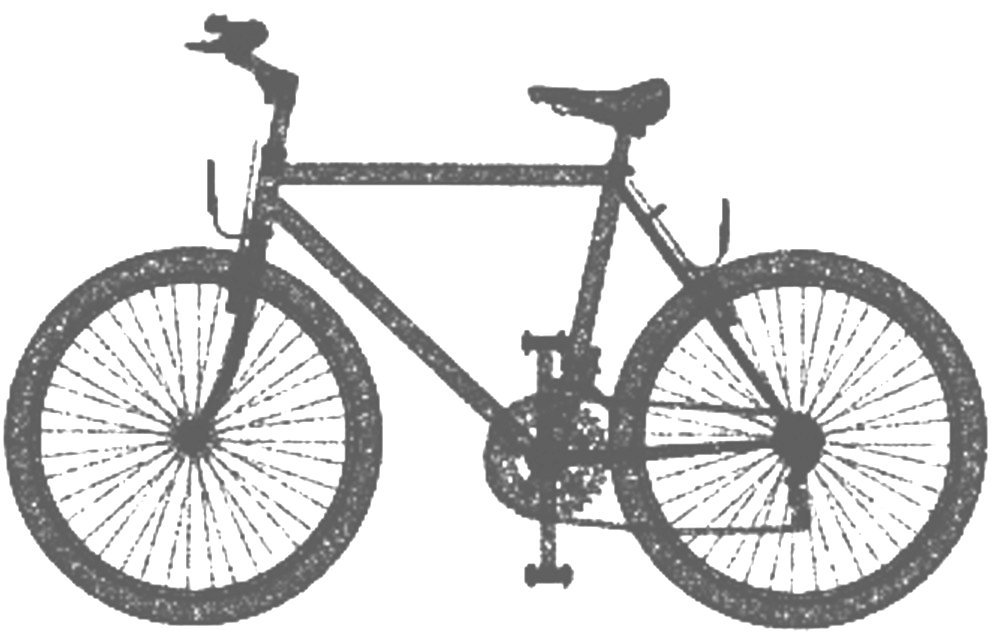
\includegraphics[width=0.175\linewidth]{./fig/eval/cycle_input.jpg} 
		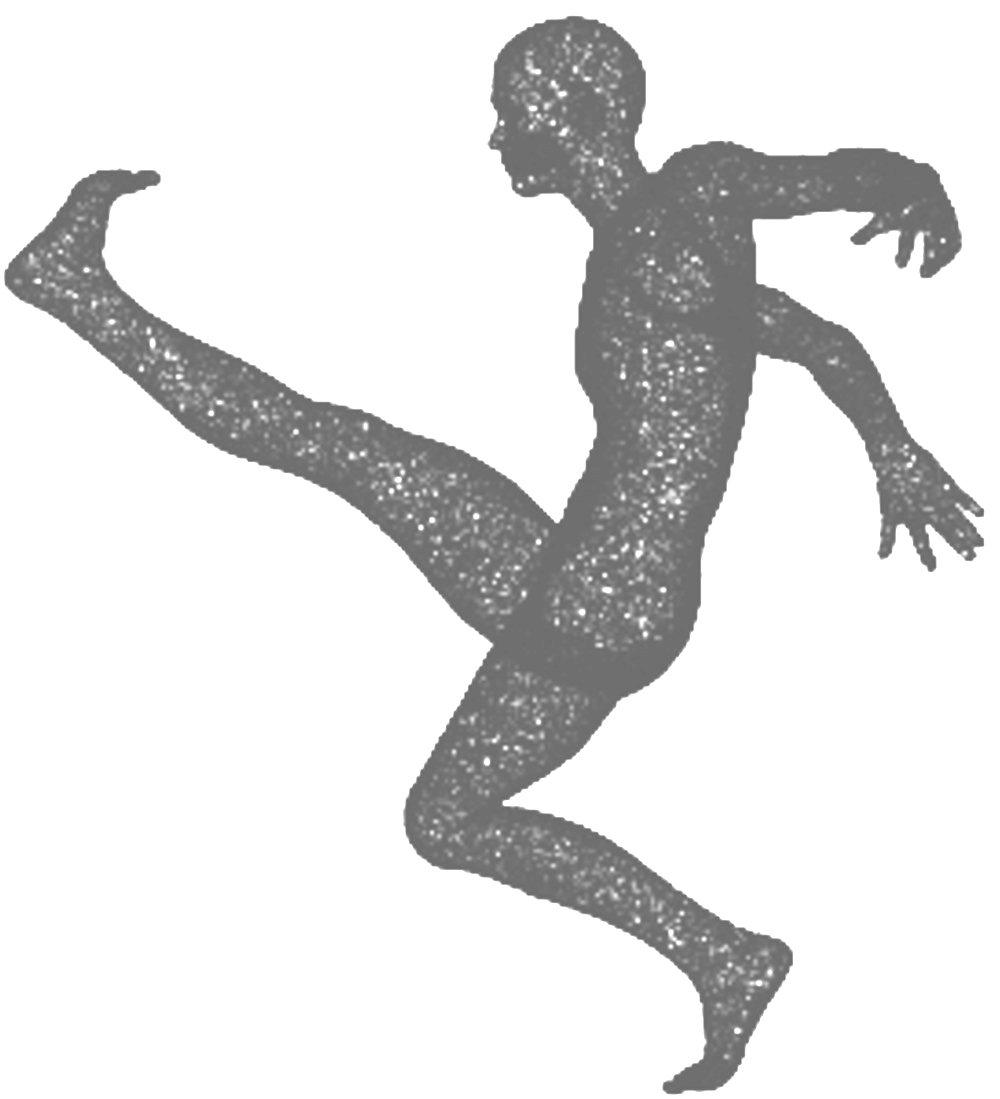
\includegraphics[width=0.155\linewidth]{./fig/eval/guy_input.jpg} 
		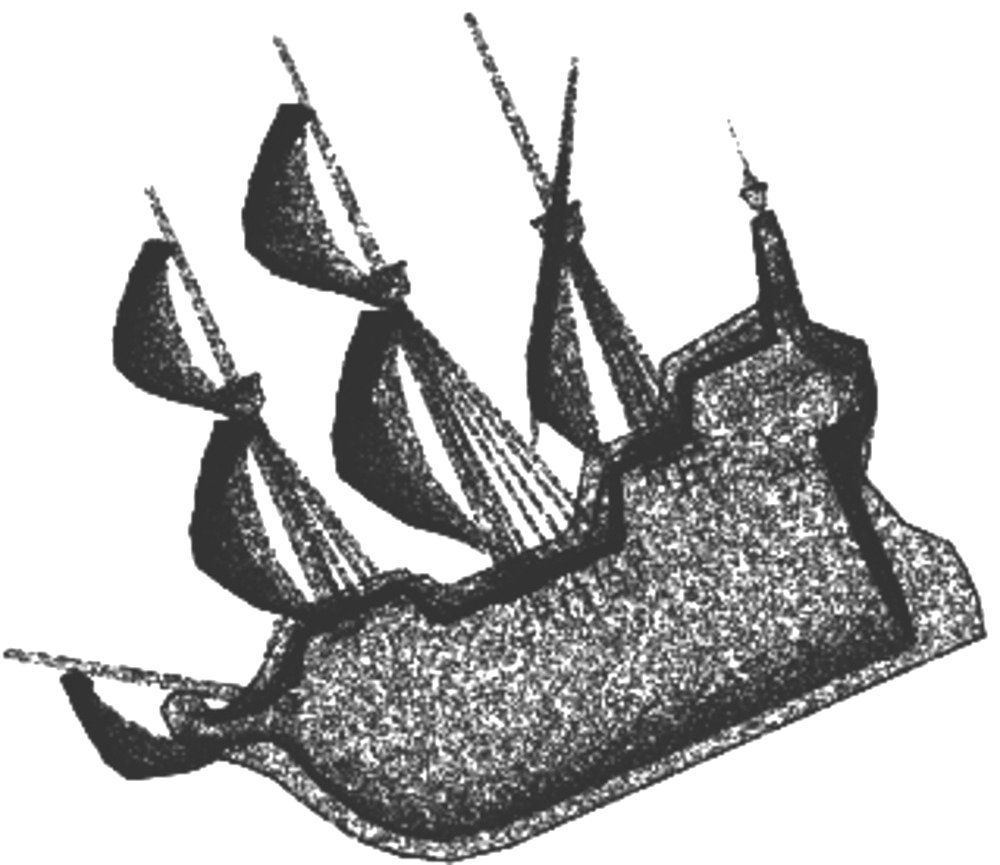
\includegraphics[width=0.175\linewidth]{./fig/eval/ship_input.jpg}
		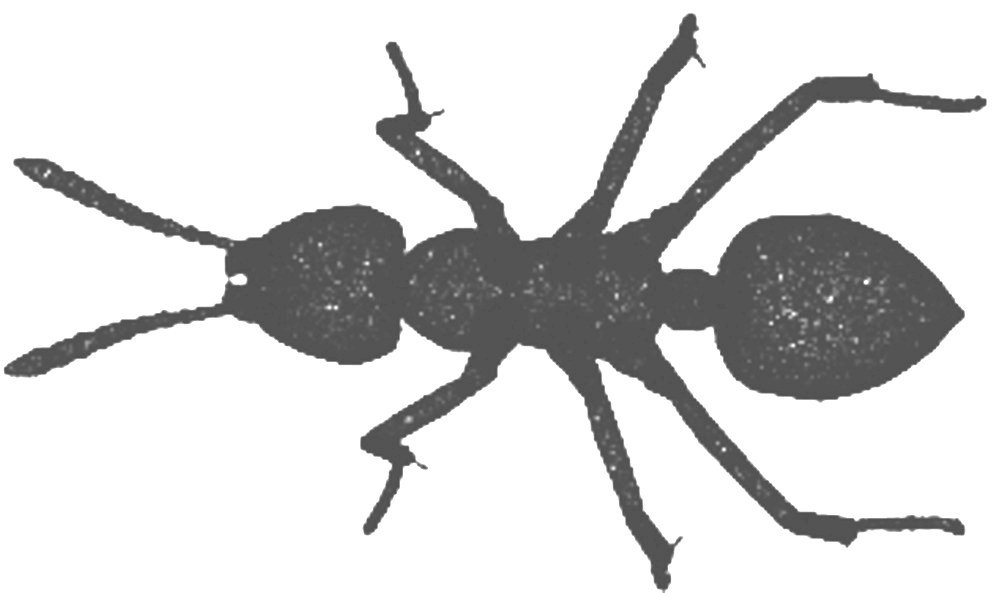
\includegraphics[width=0.175\linewidth]{./fig/eval/ant_input.jpg} 
	\end{subfigure}
	\begin{subfigure}[t]{1\linewidth} \centering 
		\phantomcaption 
		\label{fig/eval/mesh/dog}	
		\makebox[0.15\linewidth]{\raisebox{0.07\linewidth}{(b) DoG}} 
		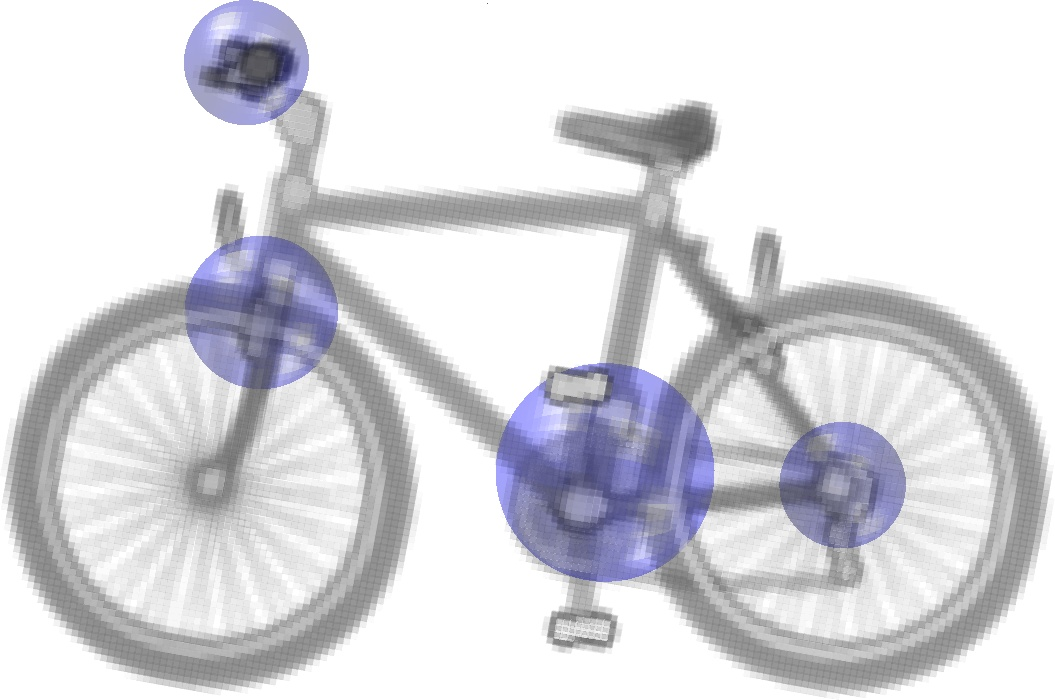
\includegraphics[width=0.175\linewidth]{./fig/eval/cycle_dog.jpg} 
		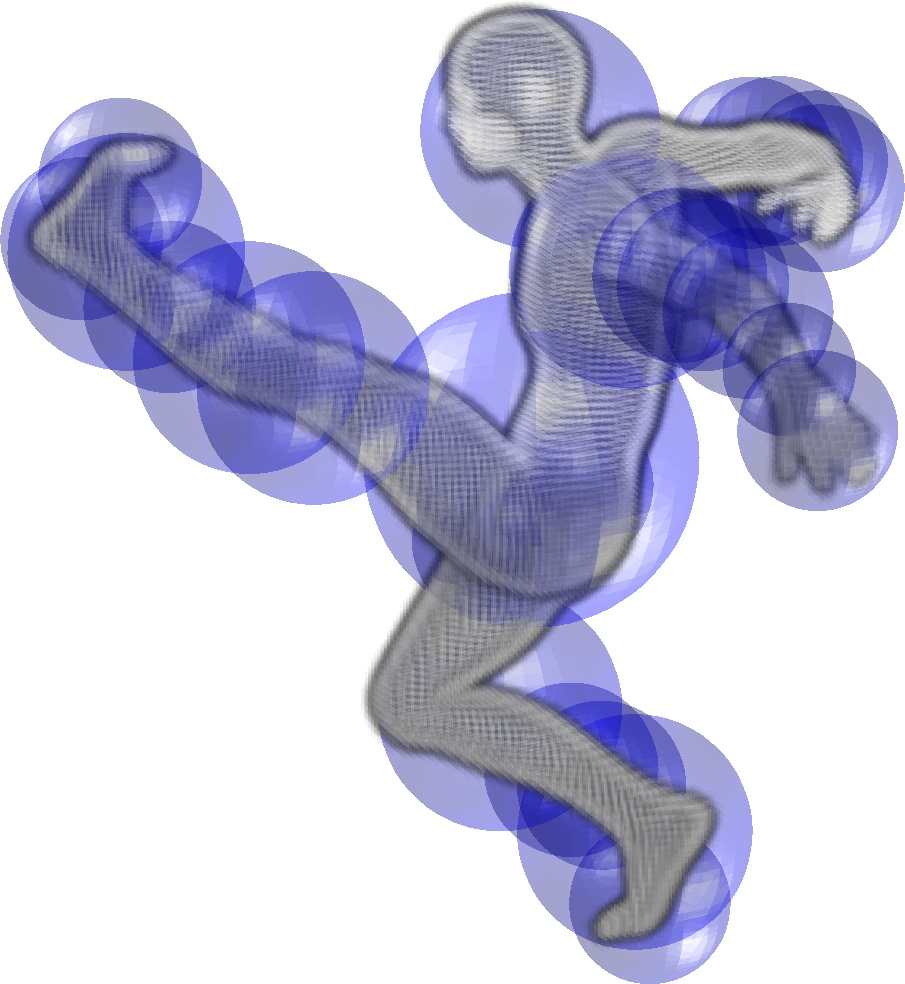
\includegraphics[width=0.155\linewidth]{./fig/eval/guy_dog.jpg} 
		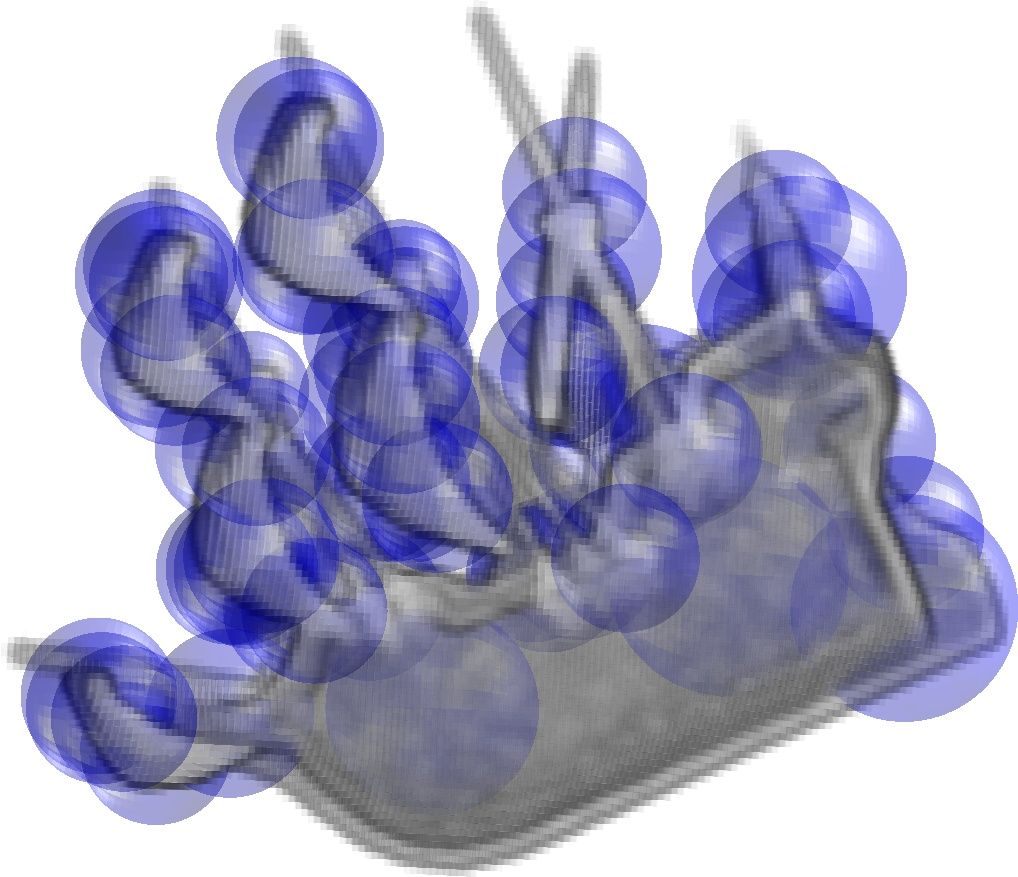
\includegraphics[width=0.175\linewidth]{./fig/eval/ship_dog.jpg}
		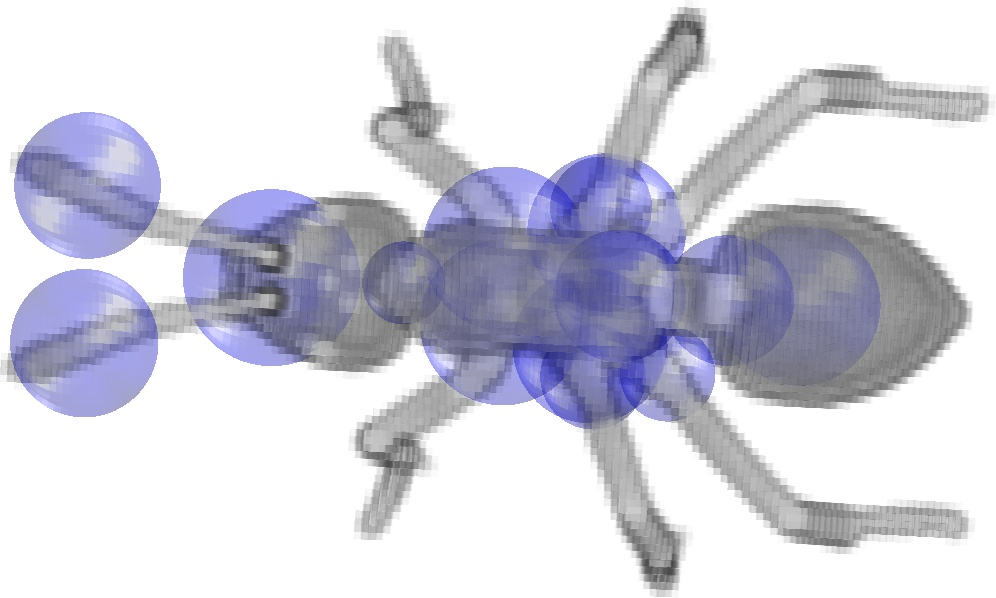
\includegraphics[width=0.175\linewidth]{./fig/eval/ant_dog.jpg} 
	\end{subfigure}
	\begin{subfigure}[t]{1\linewidth} \centering 
		\phantomcaption 
		\label{fig/eval/mesh/surf}	
		\makebox[0.15\linewidth]{\raisebox{0.07\linewidth}{(c) SURF}} 
		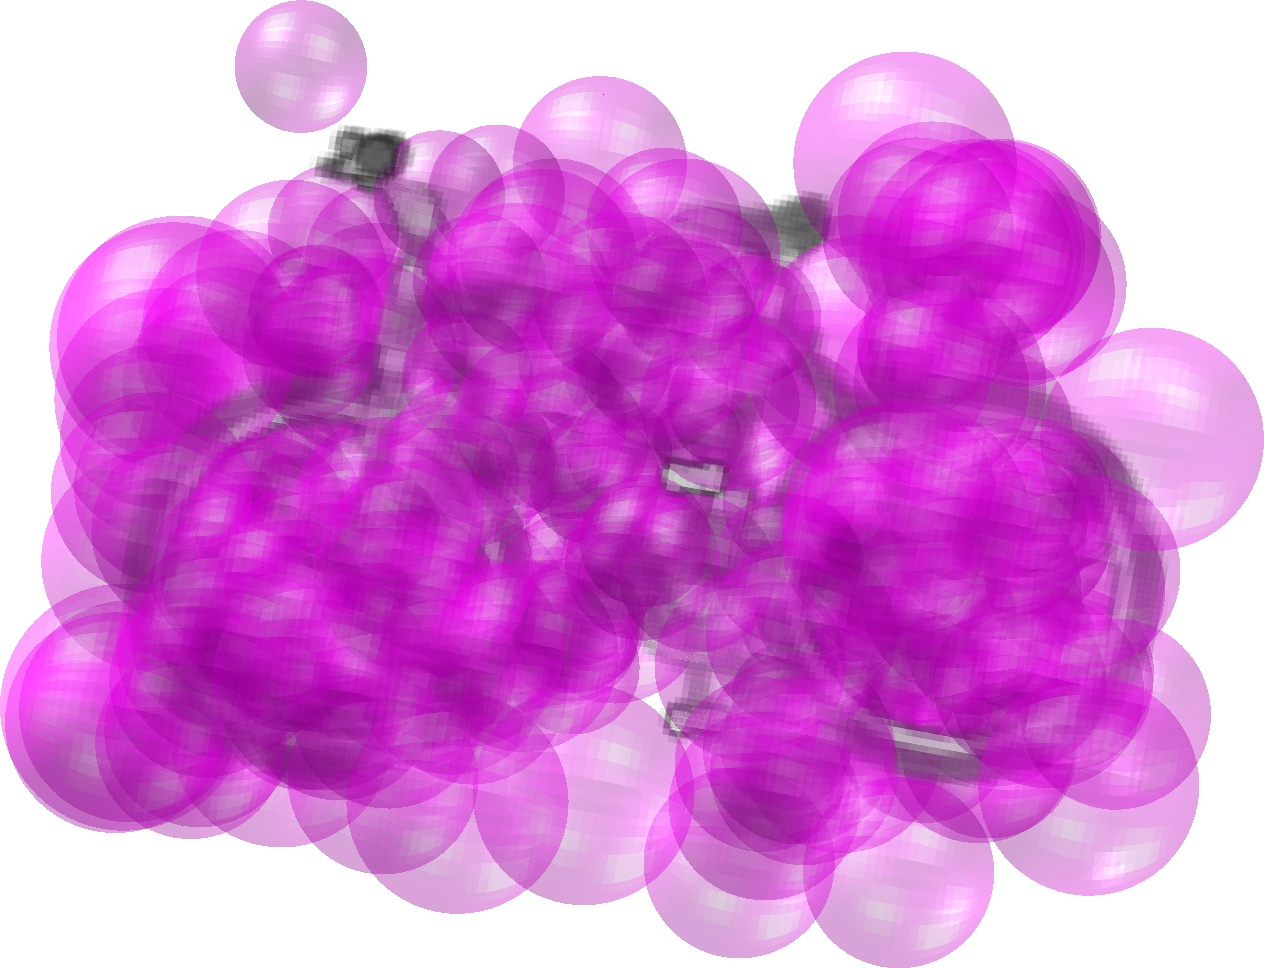
\includegraphics[width=0.175\linewidth]{./fig/eval/cycle_surf.jpg} 
		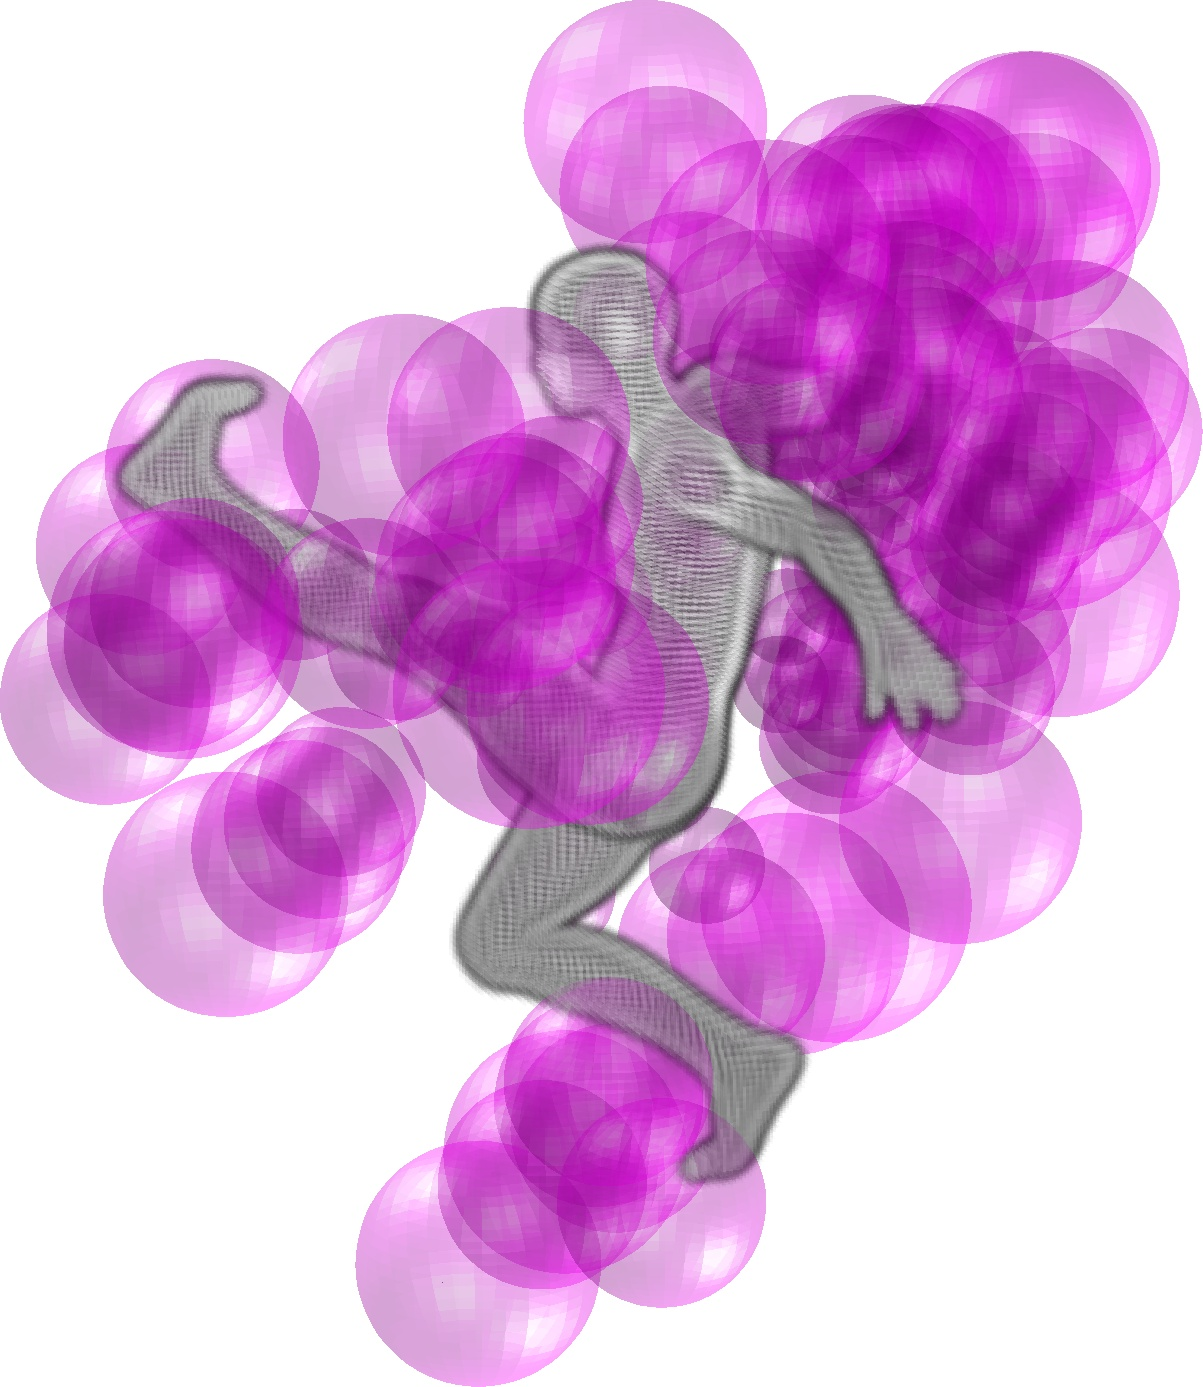
\includegraphics[width=0.155\linewidth]{./fig/eval/guy_surf.jpg} 
		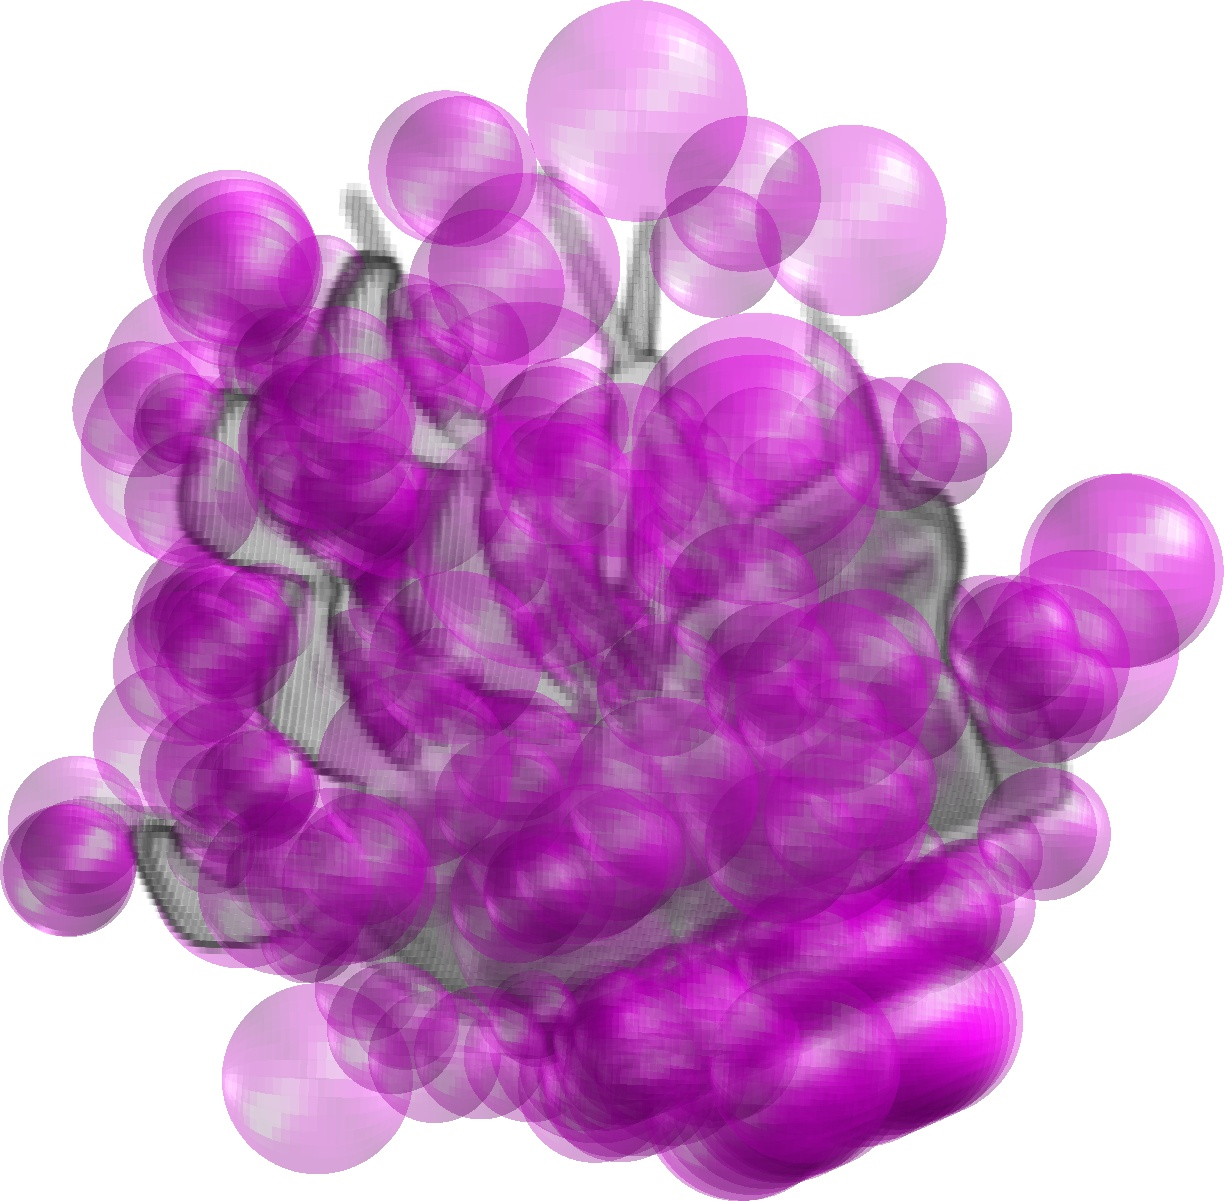
\includegraphics[width=0.175\linewidth]{./fig/eval/ship_surf.jpg}
		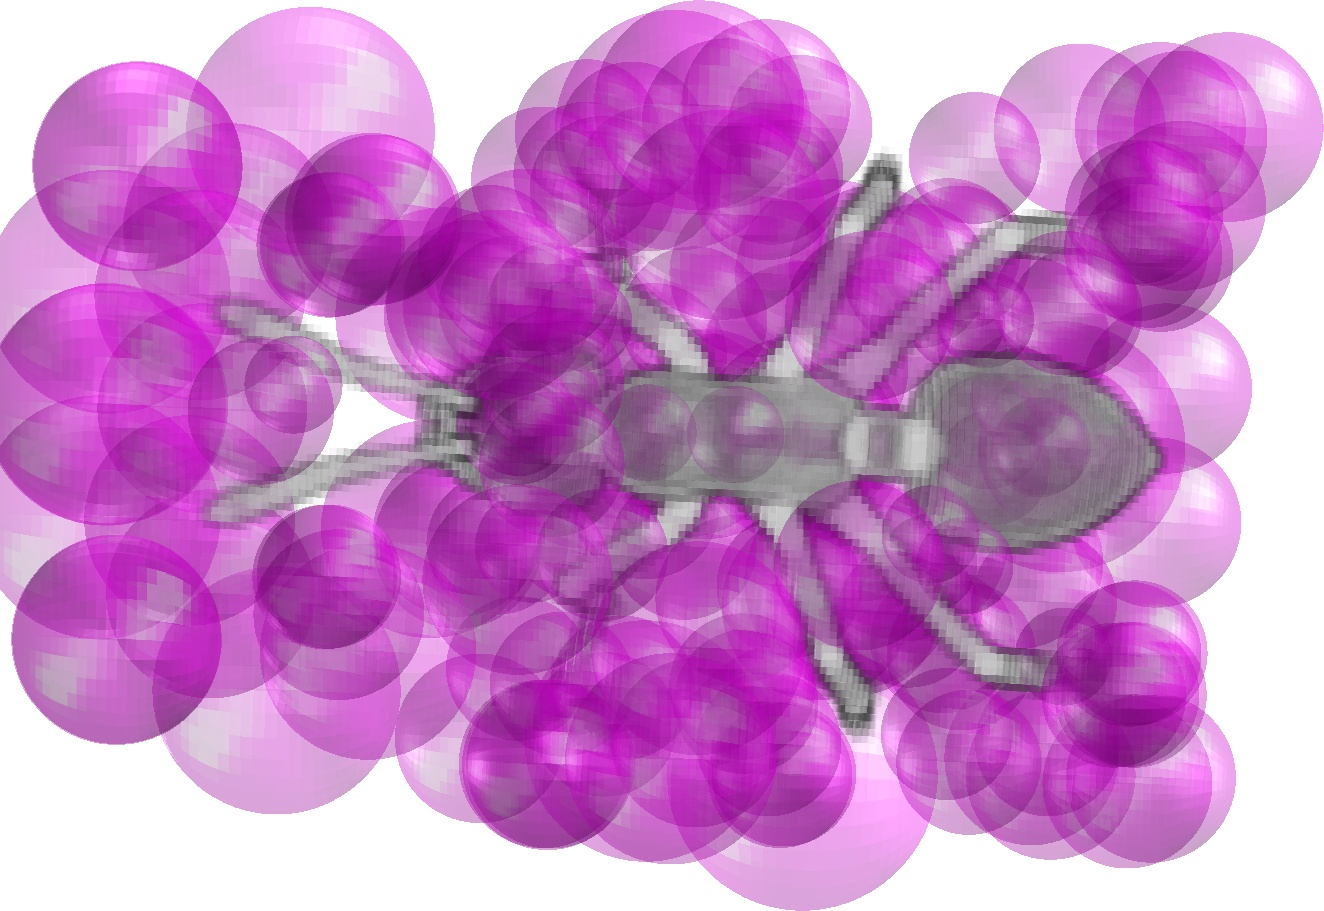
\includegraphics[width=0.175\linewidth]{./fig/eval/ant_surf.jpg} 
	\end{subfigure}
	\begin{subfigure}[t]{1\linewidth} \centering 
		\phantomcaption 
		\label{fig/eval/mesh/harris}	
		\makebox[0.15\linewidth]{\raisebox{0.07\linewidth}{(d) Harris}} 
		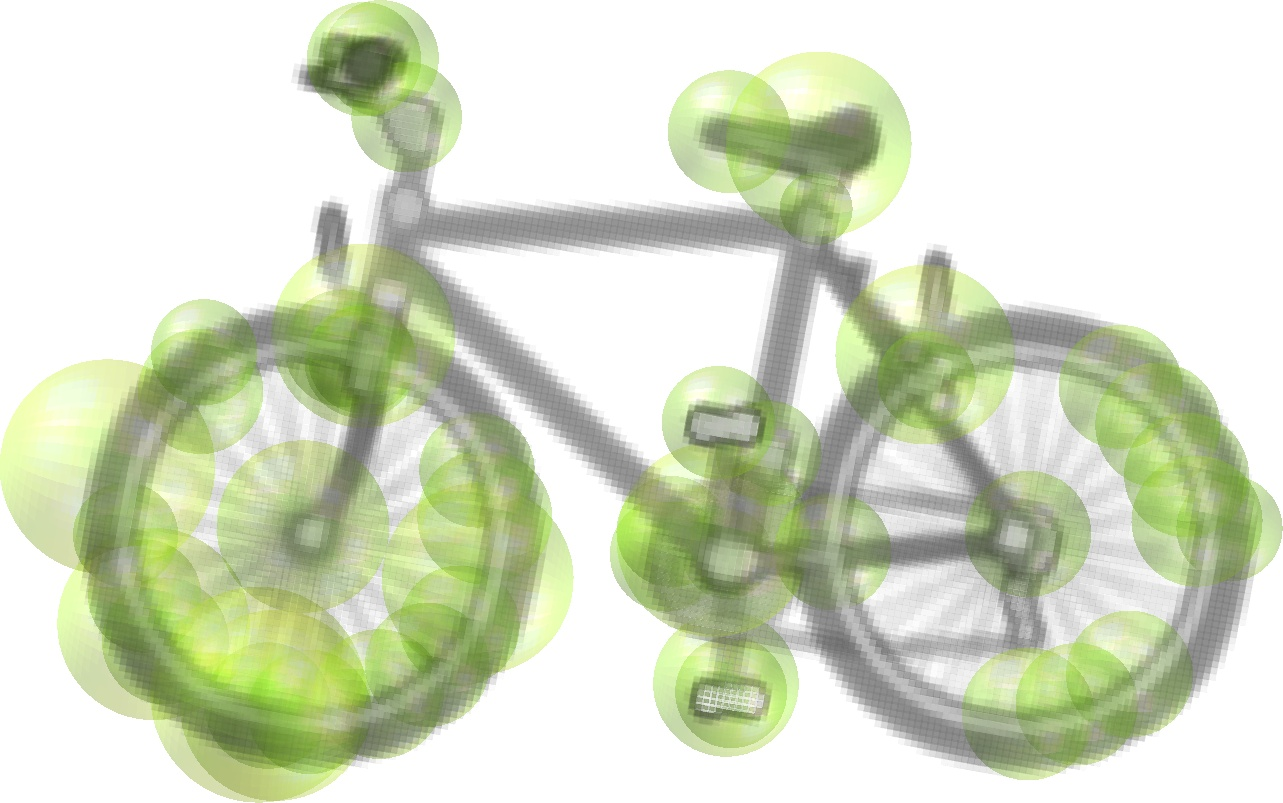
\includegraphics[width=0.175\linewidth]{./fig/eval/cycle_harris.jpg} 
		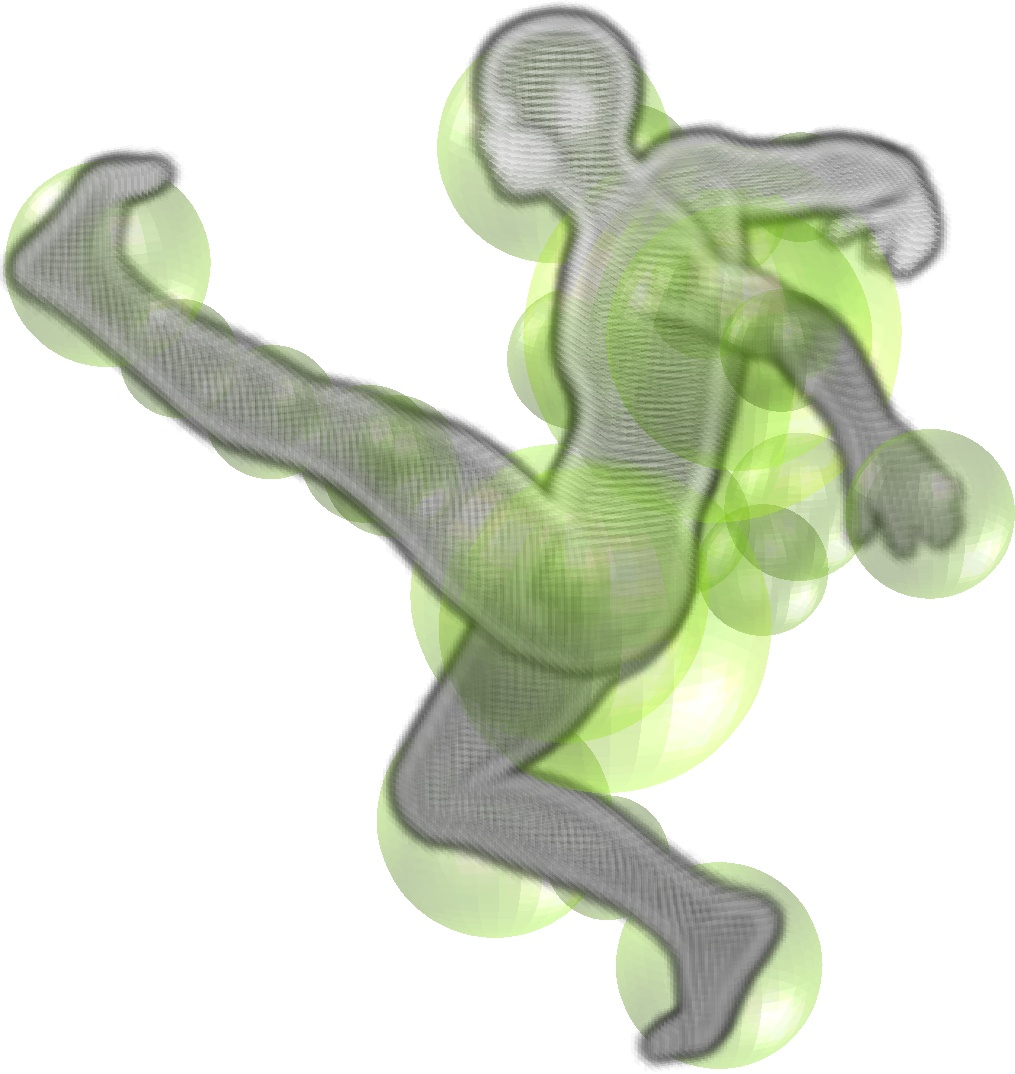
\includegraphics[width=0.155\linewidth]{./fig/eval/guy_harris.jpg} 
		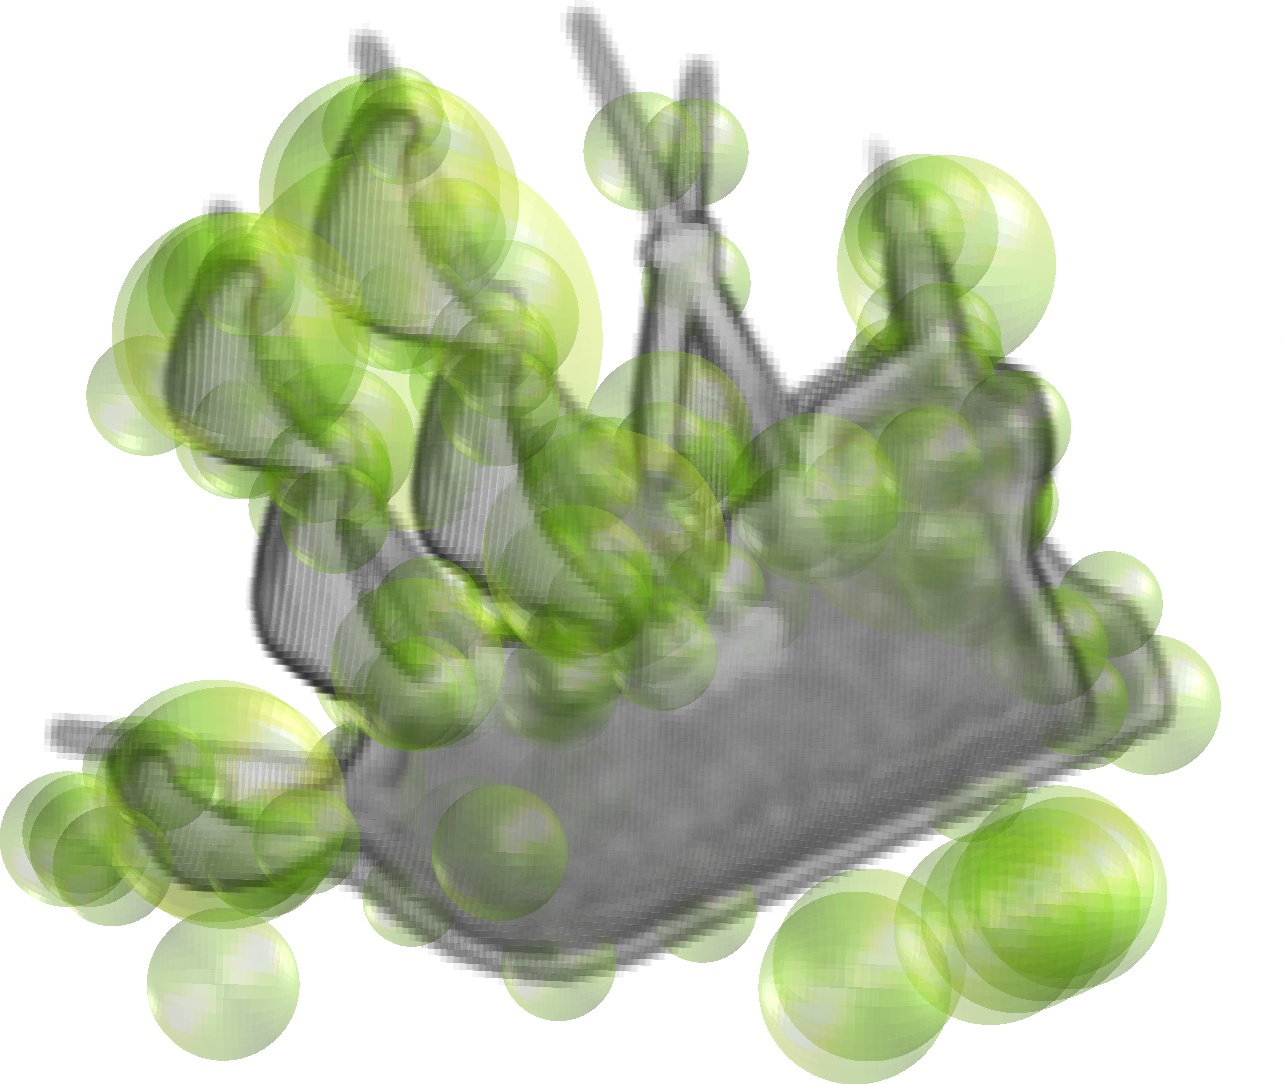
\includegraphics[width=0.175\linewidth]{./fig/eval/ship_harris.jpg}
		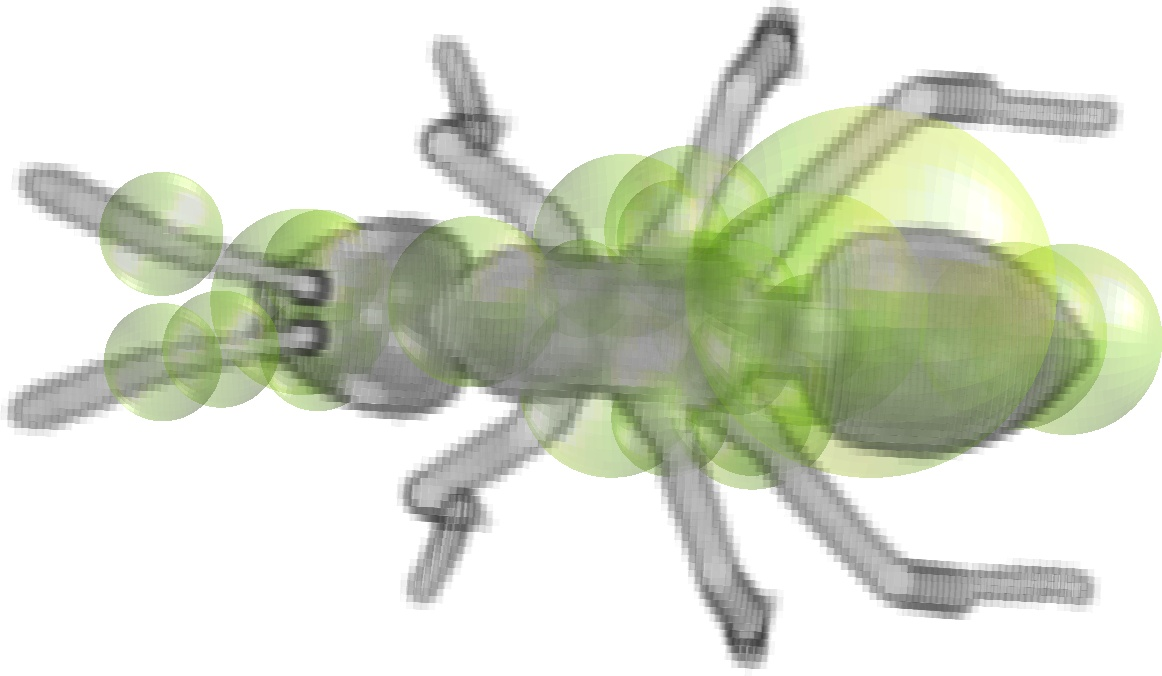
\includegraphics[width=0.175\linewidth]{./fig/eval/ant_harris.jpg} 
	\end{subfigure}
	\begin{subfigure}[t]{1\linewidth} \centering 
		\phantomcaption 
		\label{fig/eval/mesh/hessian}	
		\makebox[0.15\linewidth]{\raisebox{0.07\linewidth}{(e) DoH}} 
		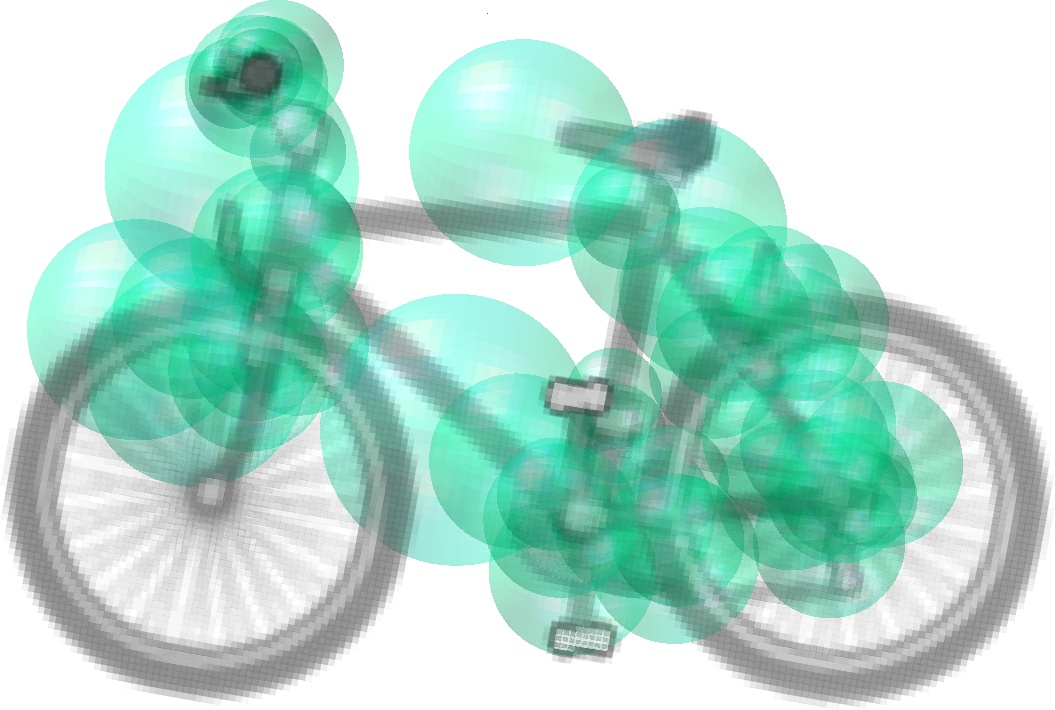
\includegraphics[width=0.175\linewidth]{./fig/eval/cycle_hessian.jpg} 
		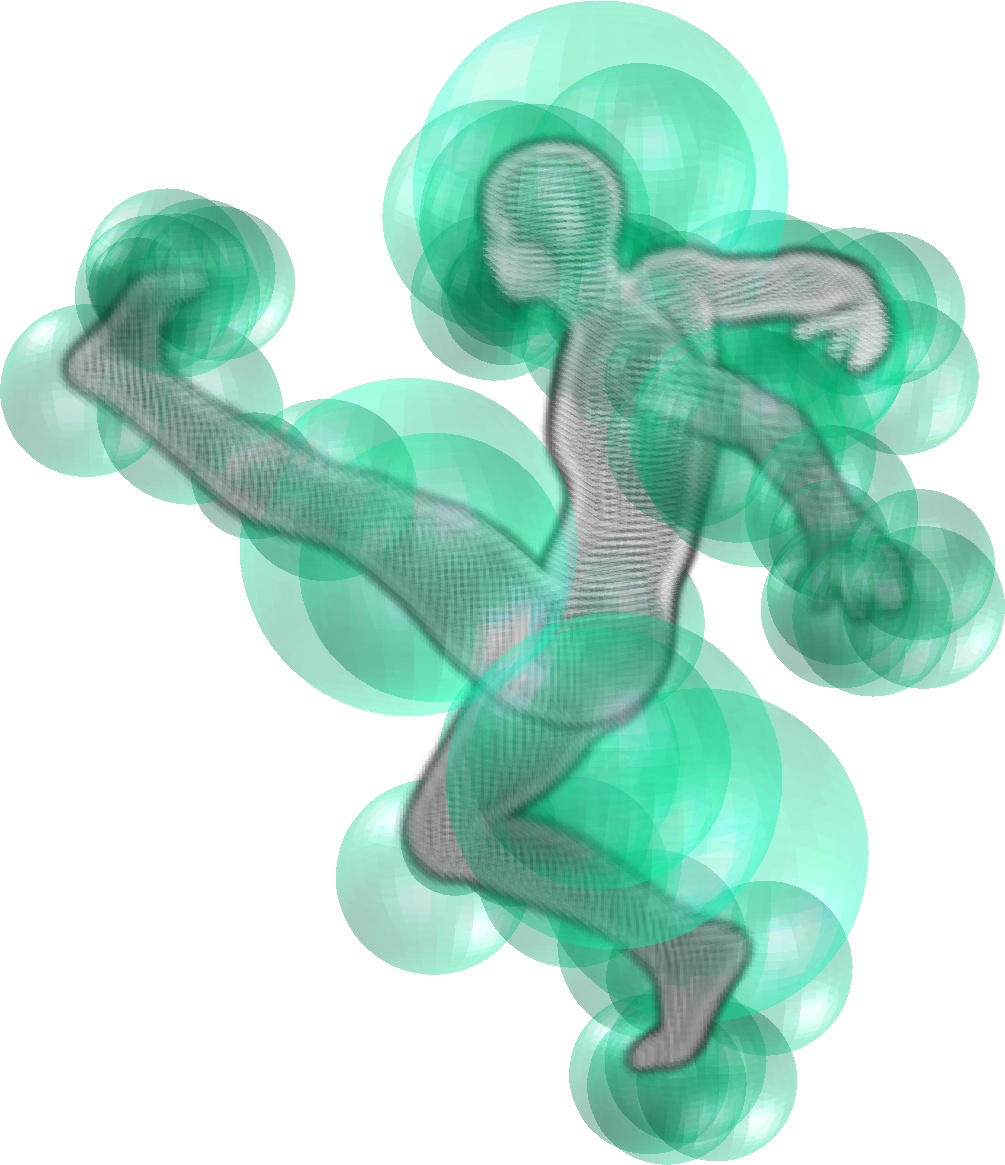
\includegraphics[width=0.155\linewidth]{./fig/eval/guy_hessian.jpg} 
		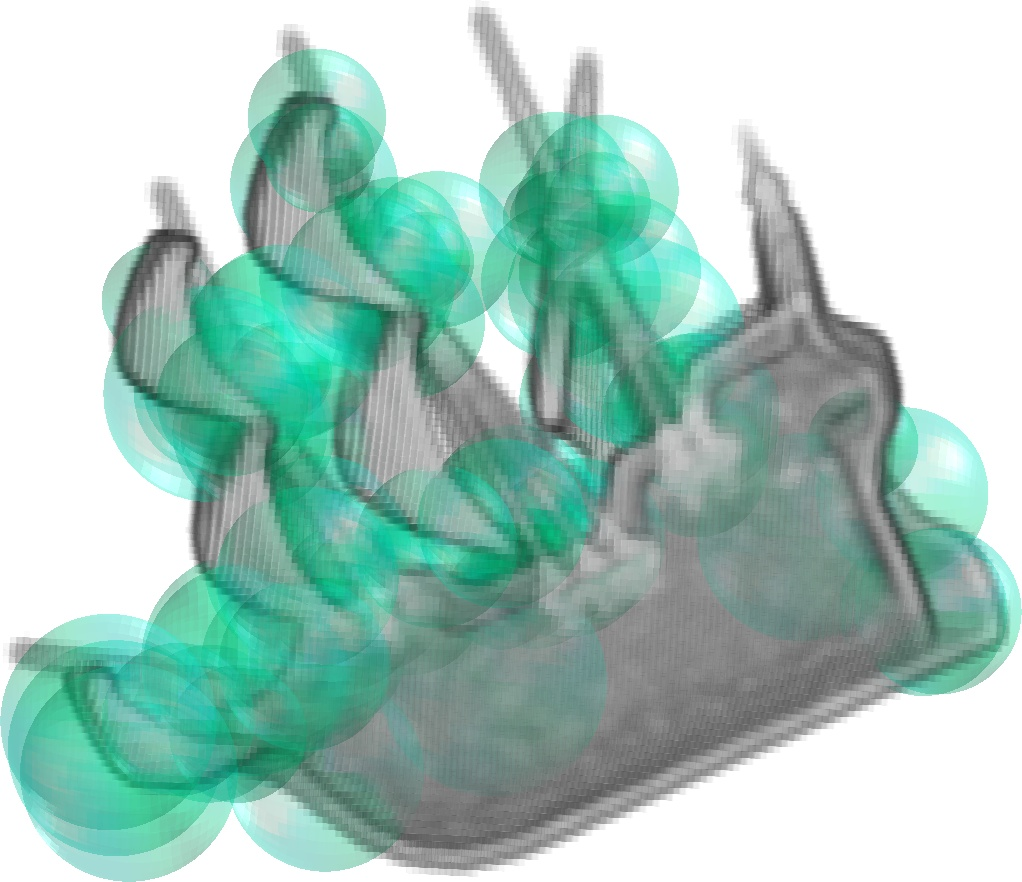
\includegraphics[width=0.175\linewidth]{./fig/eval/ship_hessian.jpg}
		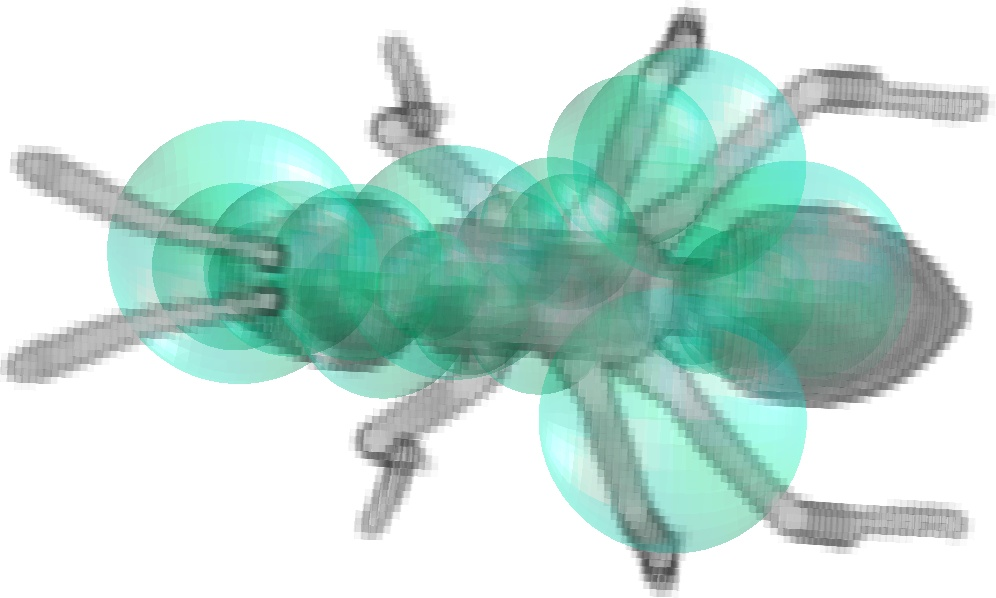
\includegraphics[width=0.175\linewidth]{./fig/eval/ant_hessian.jpg} 
	\end{subfigure}
	\begin{subfigure}[t]{1\linewidth} \centering 
		\phantomcaption 
		\label{fig/eval/mesh/fast}	
		\makebox[0.15\linewidth]{\raisebox{0.07\linewidth}{(f) VFAST}} 
		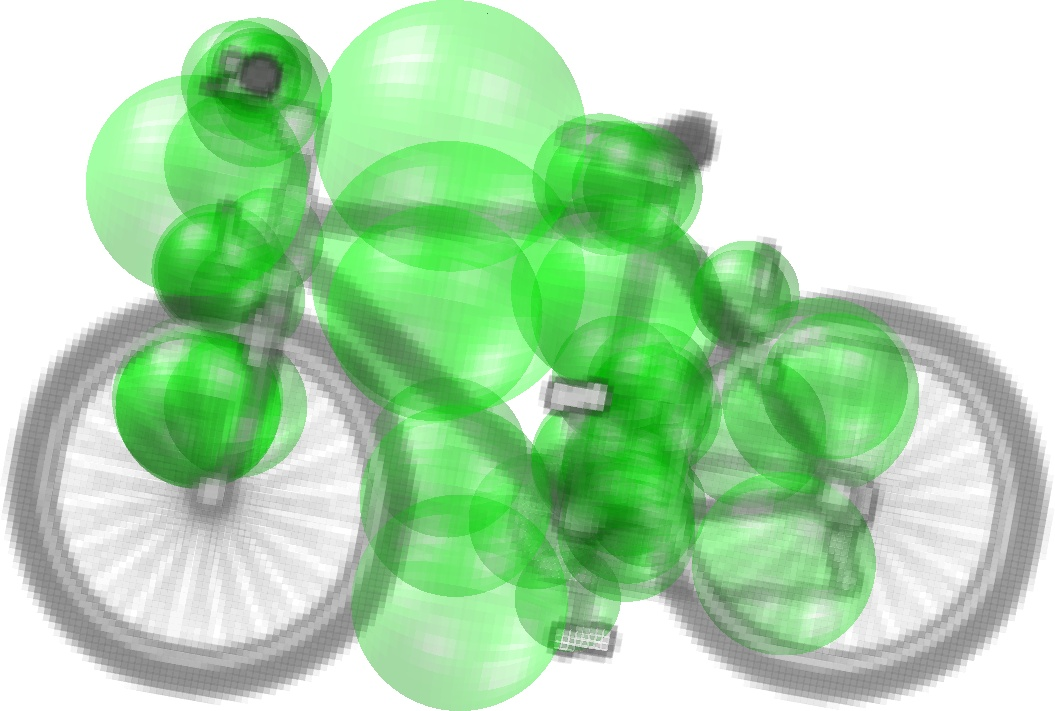
\includegraphics[width=0.175\linewidth]{./fig/eval/cycle_fast.jpg} 
		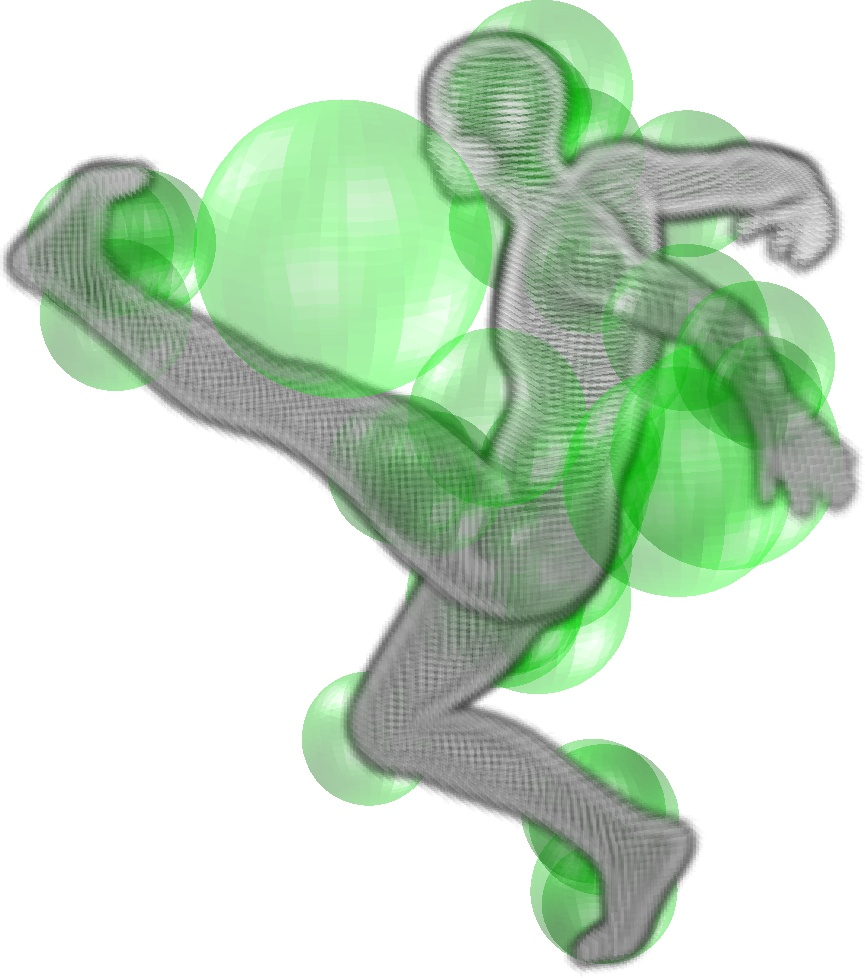
\includegraphics[width=0.155\linewidth]{./fig/eval/guy_fast.jpg} 
		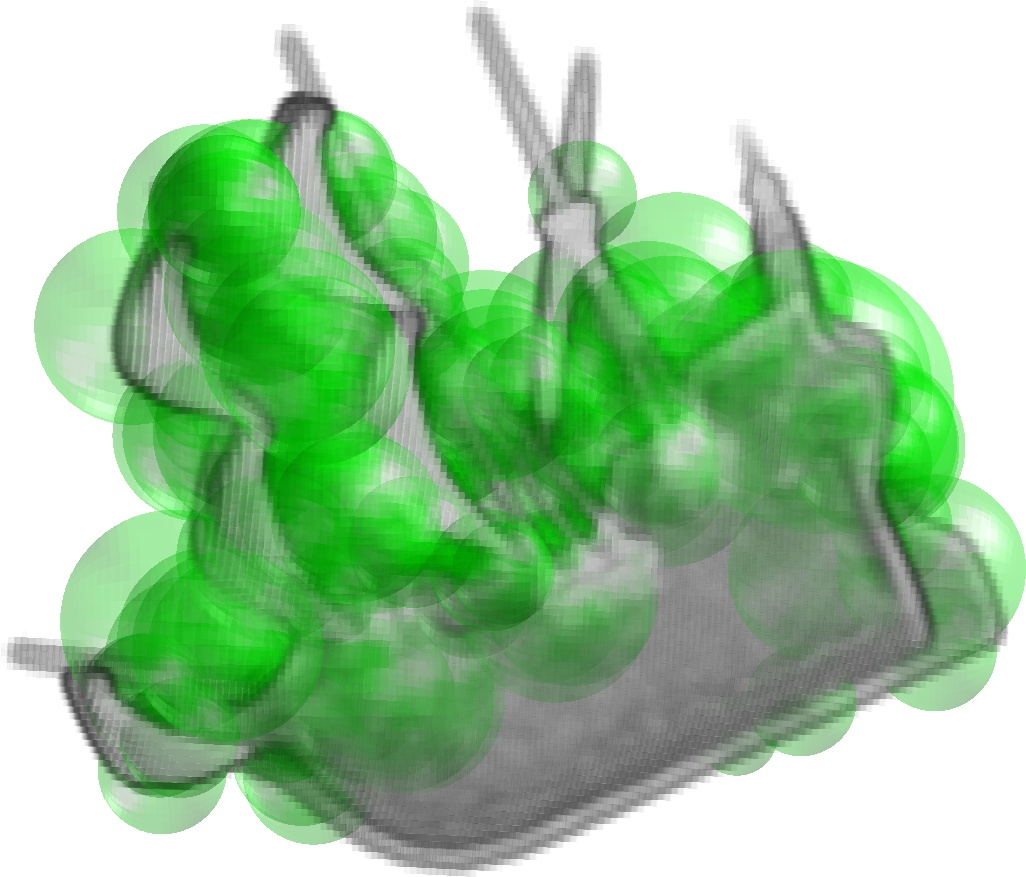
\includegraphics[width=0.175\linewidth]{./fig/eval/ship_fast.jpg}
		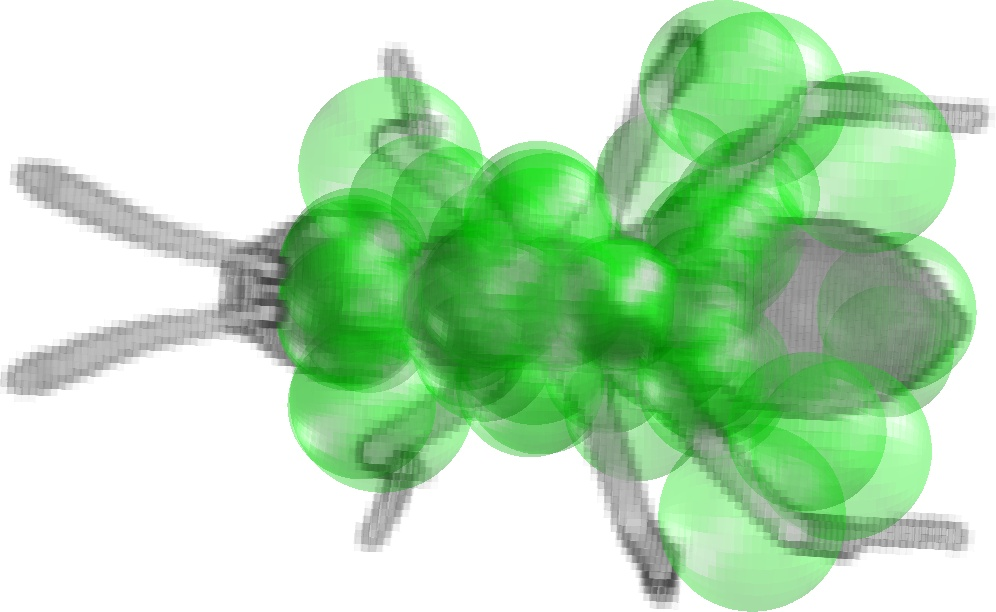
\includegraphics[width=0.175\linewidth]{./fig/eval/ant_fast.jpg} 
	\end{subfigure}
	\begin{subfigure}[t]{1\linewidth} \centering 
		\phantomcaption 
		\label{fig/eval/mesh/mser}	
		\makebox[0.15\linewidth]{\raisebox{0.07\linewidth}{(g) MSER}} 
		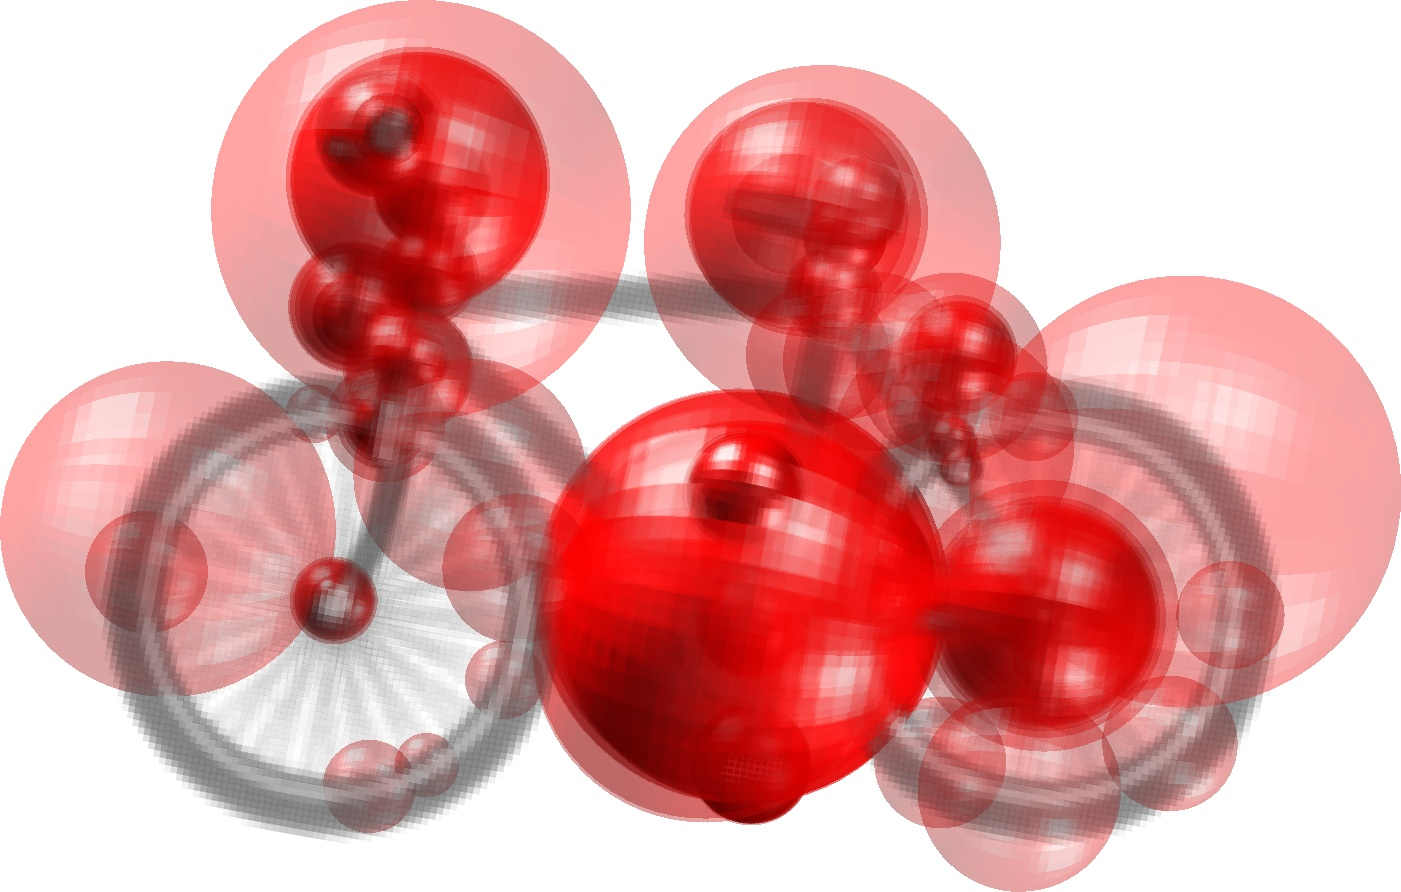
\includegraphics[width=0.175\linewidth]{./fig/eval/cycle_mser.jpg} 
		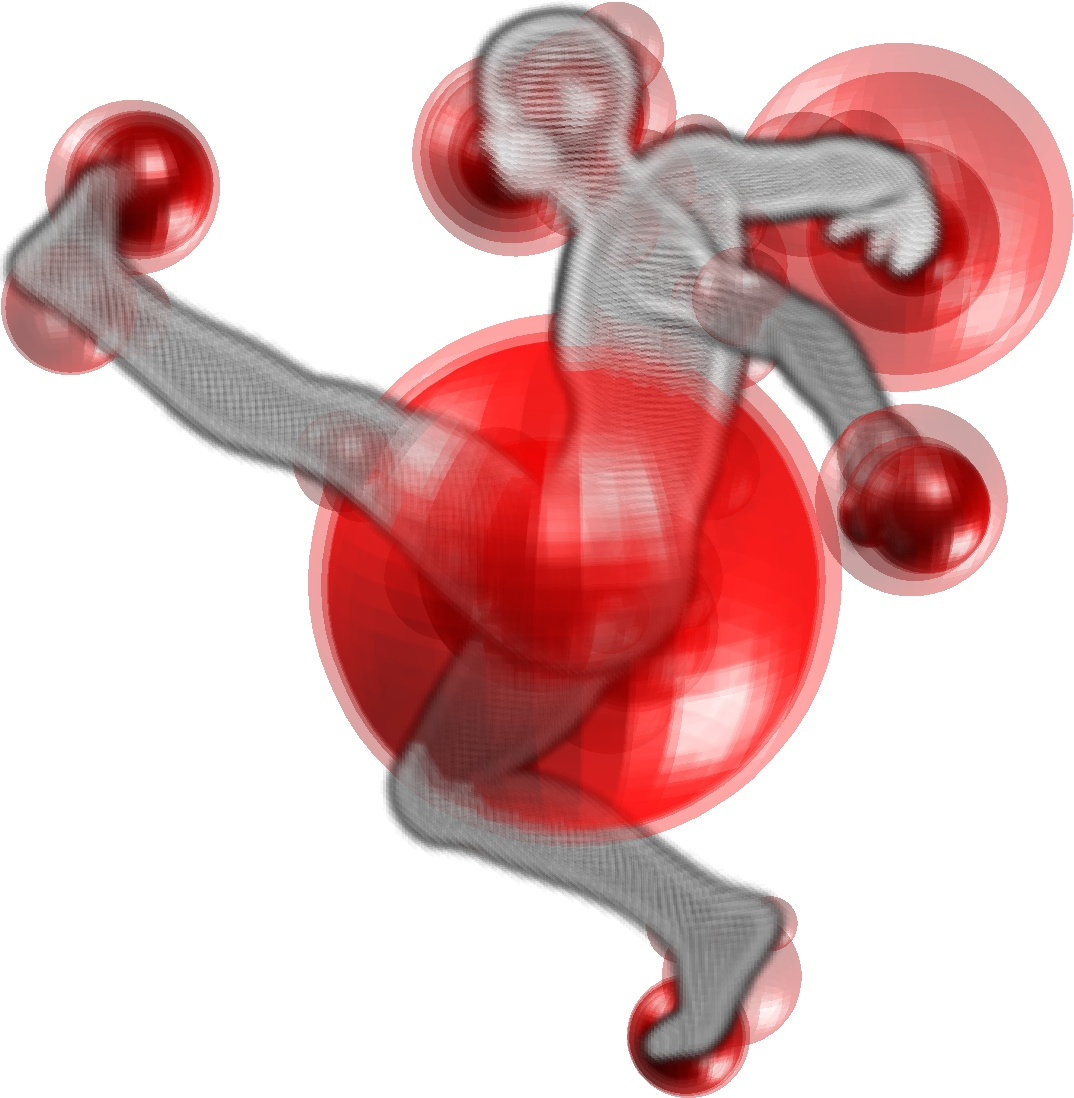
\includegraphics[width=0.155\linewidth]{./fig/eval/guy_mser.jpg} 
		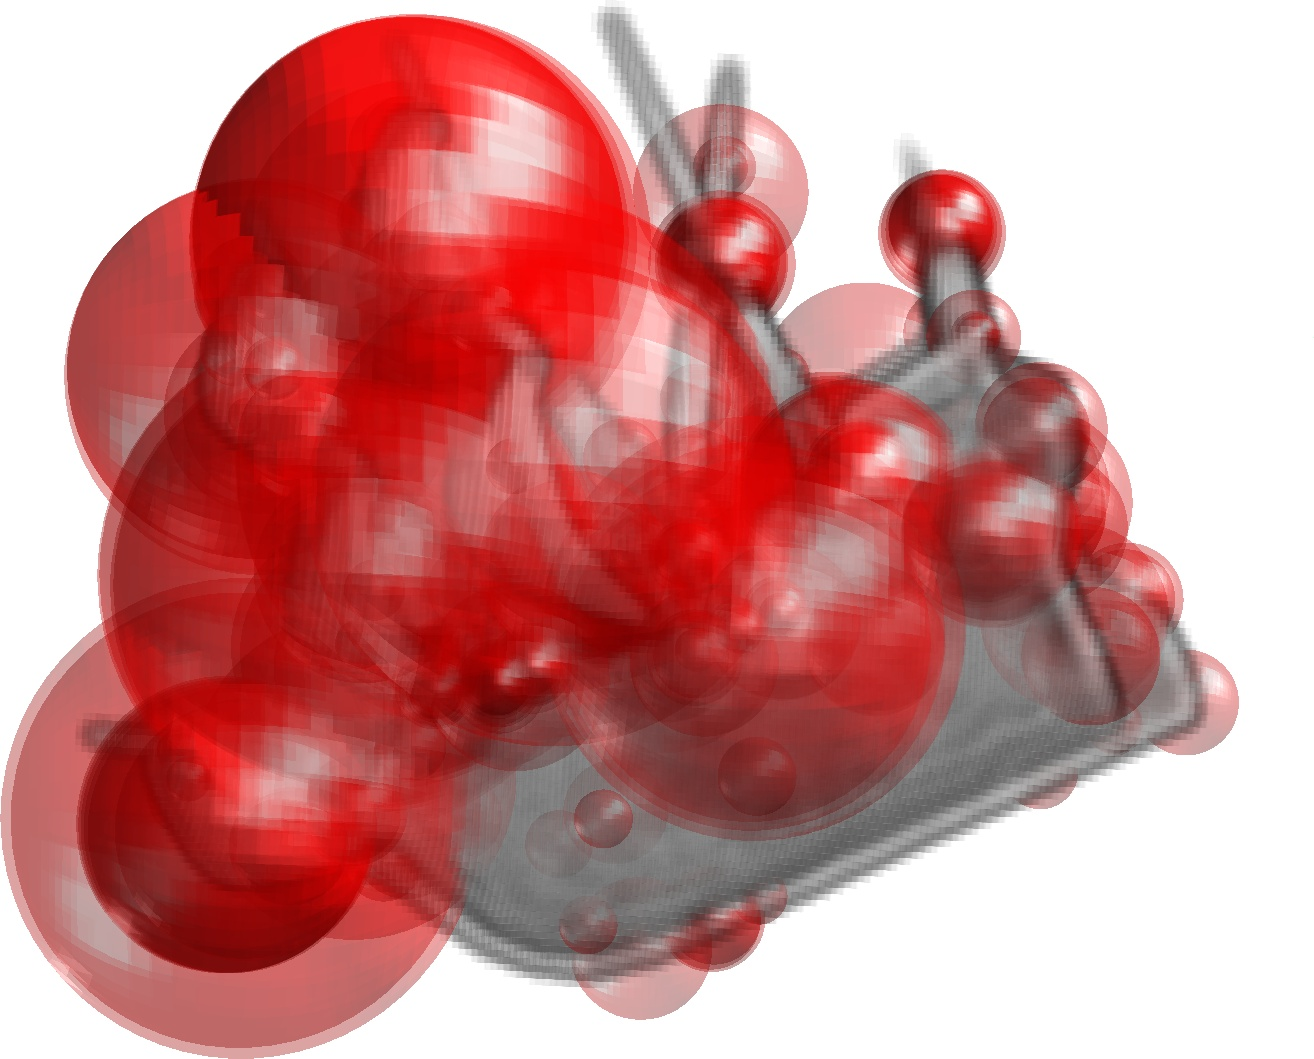
\includegraphics[width=0.175\linewidth]{./fig/eval/ship_mser.jpg}
		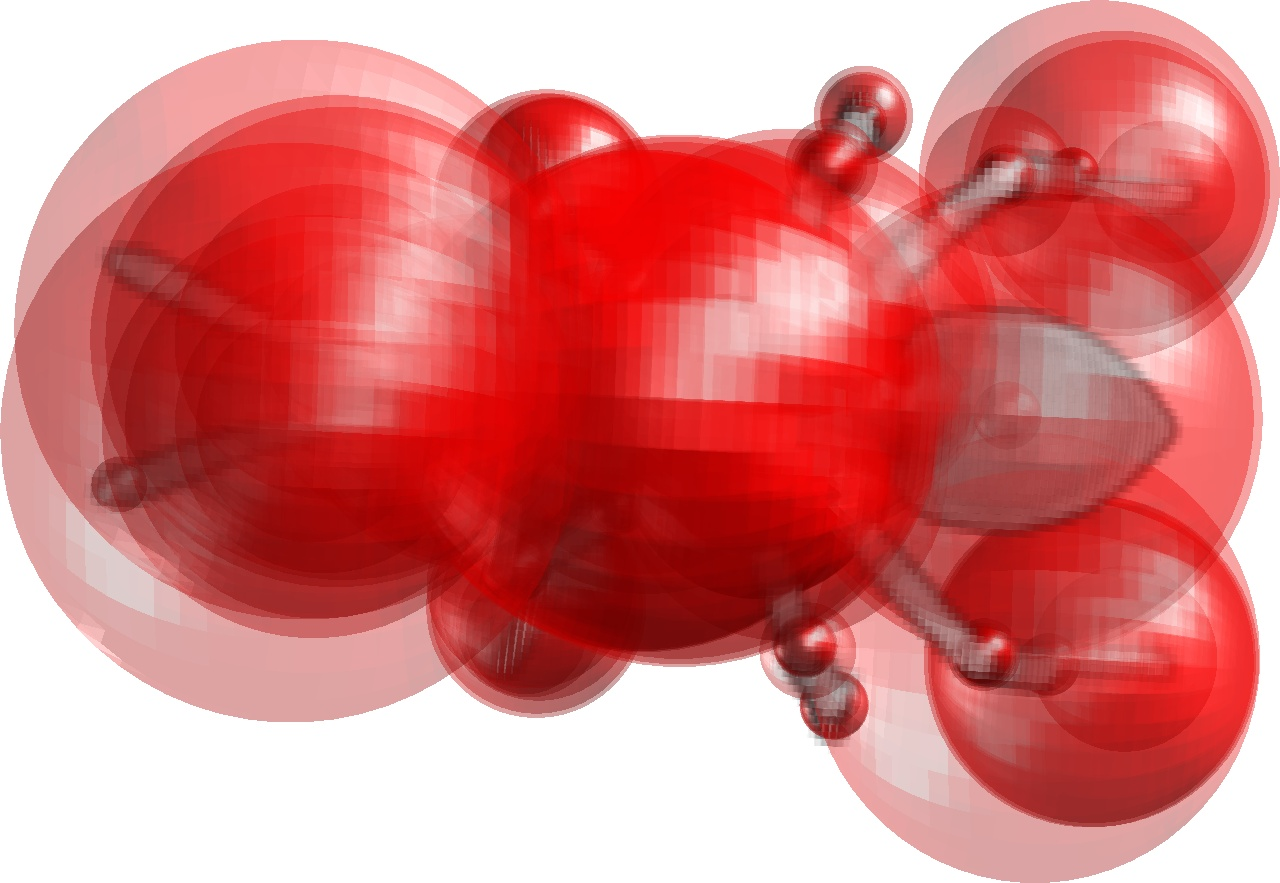
\includegraphics[width=0.175\linewidth]{./fig/eval/ant_mser.jpg} 
	\end{subfigure}
	\caption{\textbf{Interest point detection results of the \meshset dataset.} From top to bottom: (a) Sample point clouds, (b) DoG, (c) SURF (d) Harris, (e) DoH, (f) V-FAST and (g) MSER, visualized on the voxelized data. The color spheres represent the positions and relative scales of the detected interest points.}
	\label{fig/eval/mesh}
\end{figure}

